\chapter{Análise das \textit{APIs} das \textit{exchanges}}
\label{chap:desenvolvimento}

Neste capítulo são realizadas todas as análises das \textit{APIs} das corretoras de criptomoedas, baseando-se em trinta e três regras retiradas do livro \textit{REST API: Design Rulebooks} e nas limitações de uso definidas pelas próprias \textit{exchanges} na documentação de suas respectivas \textit{API}.

\section{Ferramentas utilizadas}

Nesta pesquisa foram usadas algumas ferramentas para auxiliar no processo de consulta e análise das requisições e respostas das \textit{APIs}.

\subsection{Postman}
O \textit{Postman} é uma aplicação desenvolvida com a finalidade de realizar diversos tipo de testes em \textit{APIs RESTful}. Através da sua interface, é possível enviar requisições \textit{HTTP}, analisar os resultados, consultar informações mais detalhadas e ter uma visão mais aprofundada do funcionamento dos serviços que estão sob consulta. Esta plataforma também possibilita que os desenvolvedores documentem as suas \textit{APIs} e possam planejar e escrever casos de testes.

Na imagem abaixo temos um exemplo do uso da ferramenta neste trabalho. Nele, inserimos a \textit{URI} e selecionamos o verbo \textit{HTTP} e realizamos a requisição. O \textit{software} exibirá na sua interface a resposta da requisição formatada, o cabeçalho do \textit{response}, informações do tempo de duração e do tamanho da resposta, \textit{status ode}, entre outros.
\begin{figure}[h]
	\centering
	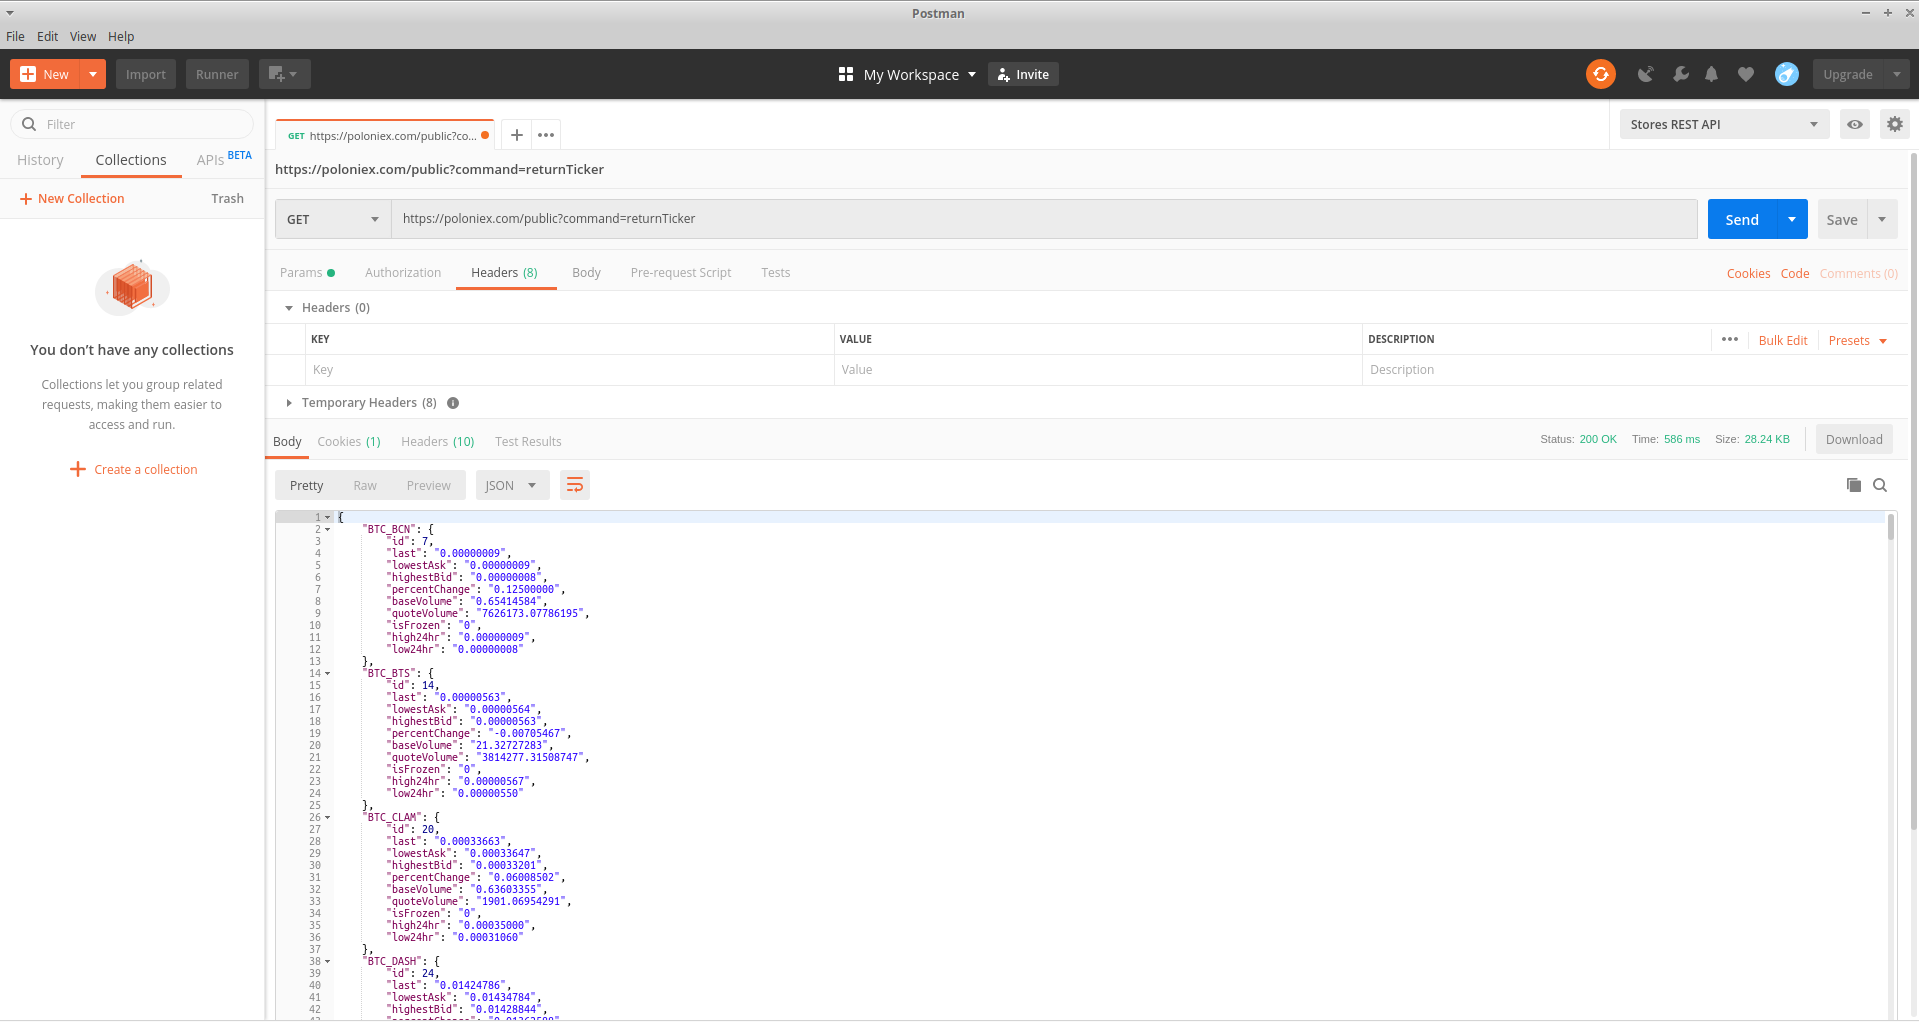
\includegraphics[width=\textwidth]{imagens/postman.png}
	\caption{Interface do Postman}
	\label{fig:postman}
\end{figure}

\subsection{Google Chrome}
O navegador Google Chrome disponibiliza em seu próprio \textit{software} as "Ferramentas de desenvolvedor", as quais permitem ao usuário analisarem uma gama de recursos e conteúdos de uma página na \textit{Internet}. Com elas, é possível ver e editar o código-fonte da página, acessar os arquivos e recursos da aplicação, visualizar as informações e dados enviadas na requisição e recebidos na resposta além de mensagens de erros, monitorar o tráfego \textit{HTTP}, depurar códigos desenvolvidos na linguagem \textit{JavaScript}, acessar informações do uso de memória e fontes de latência, entre outros.

\begin{figure}[h]
	\centering
	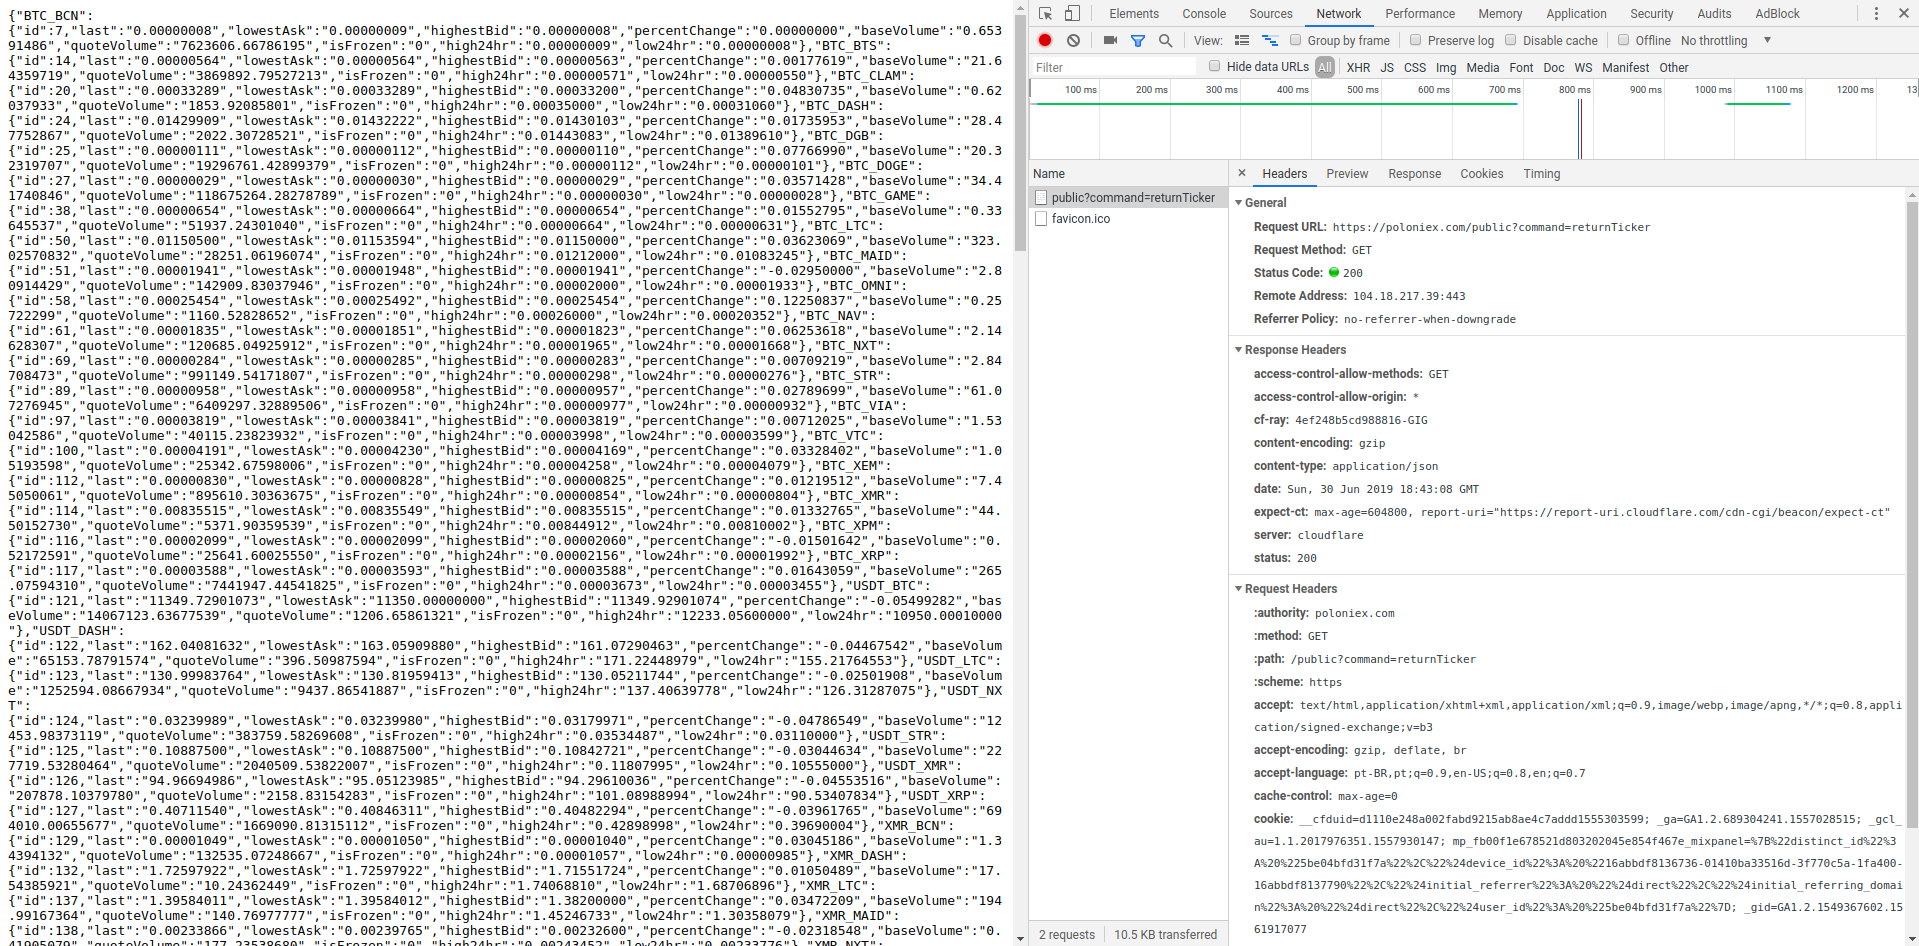
\includegraphics[width=\textwidth]{imagens/google1.png}
	\caption{Interface das Ferramentas de desenvolvedor}
	\label{fig:google}
\end{figure}

No exemplo acima é mostrado como uma requisição é feita pelo navegador e como as suas informações são dispostas na interface. No lado esquerdo a resposta é exibida ao usuário, já o lado oposto é composto pela ferramenta de desenvolvedor, com detalhes da requisição e da reposta, informações gerais - \textit{URL}, método \textit{HTTP}, \textit{status code}, etc. -, cabeçalhos do \textit{request} e do \textit{response}, além da possibilidade de ver possíveis mensagens de erro na aba \textit{Console}, informações a respeito da rede na aba \textit{Network} e dados de memória e performance.

\subsection{CURL}
O \textit{Client URL} é uma ferramenta de linha de comando, podendo também ser utilizada em \textit{scripts}, presente nos Sistemas Operacionais baseados em \textit{Unix}, e são destinados a verificar a conectividade da \textit{URL}, podendo ser utilizado também para realizar transferência de dados. Ele suporta vários protocolos utilizados na \textit{Internet}, dentre eles o \textit{HTTP}.

Em determinadas \textit{exchanges}, para acessar as rotas privadas é necessário que haja um código criptografado que é gerado através da chave privada da \textit{API}, do comando desejado e da data e hora atual em milissegundos (\textit{nonce}), utilizando o algoritmo de criptografia \textit{hash SHA-512}.   
\begin{figure}[h]
	\centering
	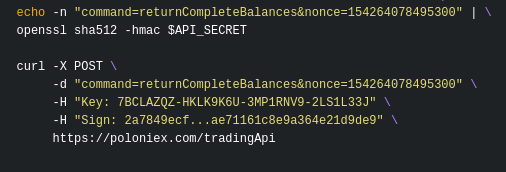
\includegraphics[width=\textwidth]{imagens/curl1.png}
	\caption{Uso do cURL}
	\label{fig:google}
\end{figure}

\section{Regras selecionadas}

\subsection{Modelagem de identificadores com \textit{URIs}}

O Identificador de Recursos Universal, ou \textit{URI} - Unified Resource Language - é um elemento presente nas \textit{APIs REST}. O mesmo é utilizado para endereçar recursos. Cada recurso deve possuir um nome significativo para que o mesmo seja identificado.
Modelá-los é uma das mais importantes tarefas para o sucesso de uma \textit{API}, sendo responsável por deixá-la mais intuitiva e de fácil manuseio para os seus usuários \cite{De2017}.

\subsubsection{Formato da \textit{URI}}

O formato de uma \textit{URI} deve seguir a seguinte estrutura abaixo:

\centerline{\textbf{esquema} "://" \textbf{autoridade} "/" \textbf{caminho} [ "?" \textbf{consulta} ] [ "\#" \textbf{fragmento} ]}

\begin{itemize}
    \item \textbf{Esquema:} É o espaço utilizado para identificar o protocolo que está sendo utilizado. Por exemplo: \textit{HTTP, HTTPS, FTP}, etc;
    \item \textbf{Autoridade:} Representa a resolução do \textit{Domain Name System} do servidor em que a aplicação está sendo executada. Pode ser composta pelo \textit{hostname} ou pelo endereço de \textit{IP}, opcionalmente com o número da porta ou com credenciais de acesso;
    \item \textbf{Caminho:} Determina uma sequência de segmentos dipostos de forma hierárquica e separados por uma barra (/);
    \item \textbf{Consulta:} São informações adicionais, não hierárquicas, de identificação. Sempre são precedidas de uma interrogação;
    \item \textbf{Fragmento:} São separados por cerquilhas (\#) e direcionam para recursos secundários dentro dos recurso primário, o qual é identificado pela autoridade.
\end{itemize}

\textbf{Regra 1 - O separador (/) deve ser usada para indicar relacionamento hierárquico.}

\begin{itemize}
    \item \textbf{Binance:} apesar de seguir a regra, algumas rotas poderiam ter uma hierarquia organizada de forma mais eficiente. Por exemplo: as rotas \textit{/api/v3/openOrders} e \textit{/api/v3/allOrders} deveriam ser atreladas a um \textit{endpoint /orders/}, que retornaria todas as ordens, e com a possibilidade eu filtrar a ordem pelo \textit{status} (aberta, finalizada, cancelada, etc.) em uma \textit{query}.
    \item \textbf{Bittrex:} utiliza a regra de forma coerente.
    \item \textbf{Poloniex:} não trabalha com hierarquia, todos os comandos são executados por meio de uma \textit{query} ou por meio do corpo da requisição utilizando \textit{JSON}.
    \item \textbf{Livecoin:} a hierarquia deveria ser melhor estruturada. Por exemplo: para as rotas \textit{/exchange/buylimit} e \textit{/exchange/selllimit}, o correto seria ter um caminho \textit{/exchange/limit} e eu escolher o tipo (\textit{buy} ou \textit{sell}) por consulta, por meio do corpo da mensagem via \textit{JSON} ou, até mesmo, criando mais duas rotas \textit{/exchange/limit/buy} e \textit{/exchange/limit/sell}.
    \item \textbf{Gate.io:} assim como na Binance e na Livecoin, o problema com a organização da hierarquia se repete. Rotas como \textit{/private/cancelOrders} e \textit{/private/cancellAllOrders} poderiam ser provenientes da hierarquia \textit{/private/orders}.
    \item \textbf{Huobi:} utiliza a regra de forma coerente.
\end{itemize}

\textbf{Regra 2 - O separador (/) não deve ser incluída no final da \textit{URI}:} o acréscimo deste elemento não adiciona nenhum conteúdo semântico e pode causar confusão.

Todas as corretoras cumprem esta regra.

\textbf{Regra 3 - Hífens (-) devem ser utilizados para melhorar a legibilidade da \textit{URI}.}

\begin{itemize}
    \item \textbf{Binance:} utiliza o padrão \textit{camelCase}, onde a primeira palavra inicia com letra minúscula e as demais com letra maiúscula.
    \item \textbf{Bittrex:} não separa as palavras.
    \item \textbf{Poloniex:} utiliza o padrão \textit{camelCase}.
    \item \textbf{Livecoin:} não possui um padrão, em determinados \textit{endpoints} faz a separação com sublinha (\_), enquanto outros são separados com o padrão \textit{camelCase}.
    \item \textbf{Gate.io:} não tem um padrão definido, alterna entre sublinhas e \textit{camelCase}.
    \item \textbf{Huobi:} padronizada com o \textit{camelCase}.
\end{itemize}

\textbf{Regra 4 - Sublinhas (\_) não devem ser usadas nas \textit{URIs}:} geralmente, aplicações de visualização de texto utilizam a sublinha para indicar que aquele elemento é clicável. Além disso, dependendo da fonte utilizada na aplicação, a sublinha pode ficar escondida ou de difícil visualização.

Como mostrado na regra de número 3, as corretoras Livecoin e Gate.io fazem uso das sublinhas, dessa forma ambas não cumprem a regra.

\textbf{Regra 5 - Letras minúsculas devem ser preferidas em caminhos da \textit{URI}:} A \textit{RFC} 3986\footnote{\em https://www.ietf.org/rfc/rfc3986.txt} define que as \textit{URIs} são \textit{case-sensitive}, ou seja, diferenciam letras minúsculas e maiúsculas nos componentes do Identificador de Recurso Universal (com exceção do esquema e da autoridade).

Apenas a Bittrex utiliza letras minúsculas em todas as suas rotas.

\textbf{Regra 6 - Extensões de arquivos não devem ser inclusas nas \textit{URIs}.} Todas as \textit{exchanges} cumprem esta regra nas suas \textit{APIs}.

\subsubsection{Modelagem de autoridade da \textit{URI}}

\textbf{Regra 7 - Nomes de subdomínios consistentes devem ser utilizados:} os nomes do domínio de alto nível e do primeiro subdomínio (ex.: ifrn.edu.br) de uma \textit{API} deve identificar o proprietário do serviço ofertado. O nome completo deve incluir um subdomínio chamado \textbf{api}, como na estrutura a seguir.

\centerline{https://api.ifrn.edu.br}

\begin{itemize}
    \item \textbf{Binance:} cumpre a regra.
    \item \textbf{Bittrex:} cumpre a regra.
    \item \textbf{Poloniex:} não segue o padrão \textit{api.subdominio}, além de possuir duas ramificações na \textit{URI}, uma para a api pública (\textit{poloniex.com/public}) e outra para a privada (\textit{poloniex.com/tradingApi}).
    \item \textbf{Livecoin:} cumpre a regra.
    \item \textbf{Gate.io:} tem quatro subdomínios, dados para os dados públicos (\textit{data.gateio.co/api2/1} e \textit{data.gateio.io/api2/1}) e mais dois para informações privadas (\textit{api.gateio.co/api2/1/private} e \textit{api.gateio.io/api2/1/private}).
    \item \textbf{Huobi:} cumpre a regra.
\end{itemize}

\subsubsection{Resumo}

\begin{table}[h]
    \centering
    \begin{tabular}{|c|c|c|c|c|c|c|}
        \hline
        \textbf{Regras} & \textbf{Binance} & \textbf{Bittrex} & \textbf{Poloniex} & \textbf{Livecoin} & \textbf{Gate.io} & \textbf{Huobi} \\ \hline
        Regra 1         & Parcialmente             & Sim                & Não                 & Parcialmente               & Parcialmente              & Sim             \\ \hline
        Regra 2         & Sim                & Sim                & Sim                 & Sim                 & Sim                & Sim              \\ \hline
        Regra 3         & Não                & Não                & Não                 & Não                 & Não                & Não              \\ \hline
        Regra 4         & Sim                & Sim                & Sim                 & Não                 & Não                & Sim              \\ \hline
        Regra 5         & Parcialmente              & Não                & Parcialmente               & Parcialmente               & Parcialmente              & Parcialmente            \\ \hline
        Regra 6         & Sim                & Sim                & Sim                 & Sim                 & Sim                & Sim              \\ \hline
        Regra 7         & Sim                & Sim                & Não                 & Sim                 & Não                & Sim              \\ \hline
    \end{tabular}
    \caption{Cumprimento das regras de modelagem de identificadores com \textit{URI} por \textit{exchange}}
    \label{tab:table-1}
\end{table}

A Huobi foi a \textit{exchange que mais seguiu os padrões de modelagem de \textit{URI}}, cumprindo cinco regras e descumprindo apenas uma. Em seguida temos a Bittrex e a Binance cumprindo cinco e quatro regras, respectivamente. As demais corretoras não tiveram um bom desempenho nessa análise, cumprindo menos de quatro regras.

É notável que nenhuma das \textit{exchanges} seguiu a terceira regra. Todas optaram por utilizar o padrão \textit{camelCase} ao invés de utilizar a separação por hífens. Apesar disso, essa violação não causará impacto na utilização das \textit{APIs}.

\subsection{Modelagem de recursos}

A modelagem de recursos é um processo semelhante à modelagem de dados em bancos relacional. Ela é ajuda a fixar alguns conceitos-chave no desenvolvimento da \textit{API}.
É de demasiada importância escolher os recursos certos e modelá-los minuciosamente, para que os consumidores da aplicação possam receber as funcionalidades, comportamentos e manutenções desejadas \cite{Subramaniam2014}.

De forma similar aos padrões de projeto (\textit{design patterns}), o projeto de recursos de uma \textit{API} é composto por quatro \textbf{arquétipos de recursos} (documento, coleção, armazenamento e controlador), os quais ajudam a comunicação se tornar mais consistente entre as estruturas e comportamentos comuns.

\begin{itemize}
    \item \textbf{Documento (\textit{document}):} representa um único recurso dentro de uma coleção. É um conceito singular semelhante a uma instância de um objeto ou registro em um banco de dados;
    \item \textbf{Coleção (\textit{collection}):} equivale a um diretório de recursos gerenciado pelo servidor. Recursos adicionais podem ser inseridos pelos usuários caso seja permitido pela coleção;
    \item \textbf{Reserva (\textit{store}):} diferente das coleções, uma reservas é um repositório de recursos gerenciado pelo cliente;
    \item \textbf{Controlador (\textit{controller}):} controladores são equivalentes à funções executáveis, possuindo parâmetros, valores de retorno, dados de entrada e de saída.
\end{itemize}

\subsubsection{Modelagem do caminho da \textit{URI}}

\textbf{Regra 8 - Substantivo no plural devem ser utilizados para nomes de coleções.}

Todas as corretoras seguem esta regra, porém, a Poloniex utilizam um padrão de nomeação das rotas que retornam coleções semelhante a uma função na programação, por exemplo: \textit{returnBalances, returnOpenOrders}.

\textbf{Regra 9 - Um verbo ou uma frase verbal deve ser utilizada para nome de controladores.}

A Binance é a única que, em algumas rotas, como a \textit{/api/v3/order}, não há um verbo ou uma frase verbal para executar controladores; no exemplo citado, para criar ou remover uma ordem.

\textbf{Regra 10 - Nomes de funções \textit{CRUD} não devem ser utilizados na \textit{URI}:} identificadores devem ser utilizados para indicar apenas recursos, nunca para indicar que funções de criar, ler, atualizar e deletar conteúdos (\textit{CRUD - create, read, update, delete}) estão sendo utilizadas.

Todas as corretoras seguiram esta regra no desenvolvimento de suas \textit{APIs}.

\subsubsection{Resumo}

Todas as corretoras cumpriram as regras de modelagem de recursos, com exceção da Binance que cumpre parcialmente a nona regra. Tal cumprimento ocorre devido ao fato das \textit{APIs} das \textit{exchanges} compartilharem funções, recursos e informações semelhantes.

\begin{table}[h]
    \centering
    \begin{tabular}{|c|c|c|c|c|c|c|}
        \hline
        \textbf{Regras} & \textbf{Binance} & \textbf{Bittrex} & \textbf{Poloniex} & \textbf{Livecoin} & \textbf{Gate.io} & \textbf{Huobi} \\ \hline
        Regra 8         & Sim                & Sim                & Sim                 & Sim                 & Sim                & Sim              \\ \hline
        Regra 9         & Parcialmente       & Sim                & Sim                 & Sim                 & Sim                & Sim              \\ \hline
        Regra 10        & Sim                & Sim                & Sim                 & Sim                 & Sim                & Sim              \\ \hline
        
    \end{tabular}
    \caption{Cumprimento das regras de modelagem de recursos por \textit{exchange}}
    \label{tab:table-2}
\end{table}

 
\subsection{Modelagem de consulta da \textit{URI}}

O componente de consulta (\textit{query}) é opcional em uma \textit{URI}. O mesmo contém um conjunto de parâmetros para serem interpretados como uma variação ou derivação do recurso determinado no caminho hierárquico do identificador. Ele fornece uma interação adicional entre o usuário e a \textit{API}, como a procura por termos específicos e filtros.

\textbf{Regra 11 - O componente de consulta de uma \textit{URI} pode ser utilizado para filtrar coleções ou reservas:} no exemplo abaixo temos uma forma de utilizar as \textit{queries} para filtrar a busca por uma coleção através de um valor específico.

\centerline{https://api.ifrn.edu.br/alunos?curso=informatica}

A regra foi cumprida por todas as \textit{exchanges}.

\textbf{Regra 12 - O componente de consulta de uma \textit{URI} dever ser usado para paginar coleções ou \textit{stores}:} o cliente deve ser capaz de utilizar as \textit{queries} para retornar coleções paginadas e resultados de reservas com os parâmetros \textit{pageSize} e \textit{pageStartIndex}, indicando a quantidade máxima de conteúdo desejado por consulta e o índice do primeiro elemento.

\centerline{https://api.ifrn.edu.br/alunos?pageSize=10\&pageStartIndex=20}

No exemplo mostrado acima, a \textit{API} retornará dez elementos, com o primeiro sendo equivalente ao vigésimo em uma consulta sem filtros de paginação, ou seja, o índice inicial será vinte.

Das seis corretoras, apenas a Binance faz uso do \textit{limit} para delimitar a quantidade de elementos retornados, mas não há \textit{queries} para paginar os resultados.

\subsubsection{Resumo}

A décima primeira regra foi cumprida por todas as \textit{exchanges}, porém, a última dessa seção, não o foi.

Há alguns motivos para os desenvolvedores dessas \textit{APIs} não se preocuparem com paginações, entre eles: a limitação geralmente ocorre utilizando-se outras informações - nome da moeda, a data e hora, etc. -, e, também, porque em algumas rotas os dados retornados em tempo real podem variar a cada milésimo de segundo e, dependendo da finalidade de quem consome a \textit{API}, o retorno de apenas uma amostra de todo o conjunto de dados pode interferir no resultado desejado, dessa forma, é melhor e mais fácil disponibilizar toda a massa de dados. 

\begin{table}[h]
    \centering
    \begin{tabular}{|c|c|c|c|c|c|c|}
        \hline
        \textbf{Regras} & \textbf{Binance} & \textbf{Bittrex} & \textbf{Poloniex} & \textbf{Livecoin} & \textbf{Gate.io} & \textbf{Huobi} \\ \hline
        Regra 11        & Sim              & Sim              & Sim               & Sim               & Sim              & Sim            \\ \hline
        Regra 12        & Não              & Não              & Não               & Não               & Não              & Não            \\ \hline
    \end{tabular}
    \caption{Cumprimento das regras de modelagem de consulta de \textit{URI} por \textit{exchange}}
    \label{tab:table-3}
\end{table}


\subsection{Modelagem de interação com \textit{HTTP}}

\textit{RESTful APIs} suportam todos os elementos e aspectos do protocolo \textit{HTTP} na sua versão 1.1, como os métodos de requisição - popularmente conhecidos como verbos \textit{HTTP} -, códigos de resposta e cabeçalhos.


\subsubsection{Métodos de requisição}

O \textit{HTTP} é composto por oito verbos:

\begin{itemize}
    \item \textit{\textbf{GET:}} utilizado para recuperar dados e informações;
    \item \textit{\textbf{POST:}} tem como função enviar dados para o servidor;
    \item \textit{\textbf{PUT:}} substitui todas as informações do recurso destinado com o conteúdo submetido;
    \item \textit{\textbf{PATCH:}} similar ao \textit{PUT}, a diferença é que o \textit{PATCH} faz uma atualização parcial de um recurso, ou seja, apenas alguns atributos do recurso em questão podem ser especificados para atualização;
    \item \textit{\textbf{HEAD:}} possui a mesma funcionalidade do método \textit{GET}, porém, o servidor deve retornar na resposta apenas o cabeçalho e o \textit{status} e não o corpo da mensagem;
    \item \textit{\textbf{DELETE:}} remove a representação do recurso alvo;
    \item \textit{\textbf{OPTIONS:}} descreve as opções de comunicação com o recurso alvo;
    \item \textit{\textbf{CONNECT:}} inicia a comunicação bidirecional com o recurso alvo, estabelecendo um túnel com o servidor;
    \item \textit{\textbf{TRACE:}} realizar um teste, enviando uma mensagem pelo caminho até o recurso alvo e o servidor respondendo a mensagem recebida.
\end{itemize}

\textbf{Regra 13 - \textit{GET} deve ser utilizada para recuperar a representação de um recurso.}

Todas as \textit{exchanges} seguem a regra, a única observação é a respeito da Bittrex, que utiliza apenas o \textit{GET} para todas as rotas.

\textbf{Regra 14 - \textit{GET} e \textit{POST} não devem ser usados no lugar de outros métodos de requisição.}

\begin{itemize}
    \item \textbf{Binance:} utiliza corretamente ambos os verbos.
    \item \textbf{Bittrex:} utiliza o \textit{GET} para todas as requisições.
    \item \textbf{Poloniex:} usa o \textit{GET} corretamente, mas o \textit{POST} é utilizado no lugar do \textit{DELETE}.
    \item \textbf{Livecoin:} usa o \textit{GET} corretamente, porém, o \textit{DELETE} é substituído pelo \textit{POST}.
    \item \textbf{Gate.io:} usa o \textit{GET} corretamente, mas o \textit{POST} é utilizado no lugar do \textit{DELETE}.
    \item \textbf{Huobi:} usa o \textit{GET} corretamente, porém, o \textit{DELETE} é substituído pelo \textit{POST}.
\end{itemize}

\textbf{Regra 15 - \textit{POST} deve ser usado para criar novos recursos em uma \textit{collection}.}

A única exceção à esta regra é a Bittrex, pelo motivo citado nas duas últimas regras.

\textbf{Regra 16 - \textit{POST} deve ser utilizado para executar controladores.}

A Bittrex é a única que não cumpriu.

\textbf{Regra 17 - \textit{DELETE} deve ser utilizado para remover um recurso.}

Apenas a Binance cumpriu a regra. Todas as outras atribuíram esta funcionalidade ao \textit{GET} ou ao \textit{POST}.

\subsubsection{\textit{Status codes} de resposta}

O protocolo \textit{HTTP} define uma gama de códigos de estado para que sejam usados a fim de transmitir para o cliente os resultados de uma requisição. Os \textit{status codes} são subdivididos em cinco categorias:

\begin{itemize}
    \item \textbf{Informacionais:} retorna informações de transferência a nível de protocolo. Sempre iniciam com o número 1;
    \item \textbf{Sucesso:} indica que a requisição foi aceita com sucesso. Iniciam com o número 2;
    \item \textbf{Redirecionamento:} informa ao cliente que ele deve executar mais ações para que sua requisição seja completada. Os códigos desta categoria começam com o número 3;
    \item \textbf{Erro no cliente:} indica que o erro na resquisição aconteceu do lado do cliente. Sempre iniciam com o número 4;
    \item \textbf{Erro no servidor:} indica que o erro na resquisição aconteceu do lado do servidor. Sempre iniciam com o número 5;
\end{itemize}

\textbf{Regra 18 - 200 (\textit{"Ok"}) deve ser usado para indicar sucesso não específico.}

Regra cumprida pelas \textit{APIs} de todas as \textit{exchanges}.

\textbf{Regra 19 - 200 (\textit{"OK}) não deve ser utilizado para comunicar erros no corpo da resposta.}

\begin{itemize}
    \item \textbf{Binance:} respeita a regra, retorando o código de erro equivalente ao problema e uma mensagem com um código de erro próprio e uma descrição.
    \item \textbf{Bittrex:} em alguns casos retorna o código 200.
    \item \textbf{Poloniex:} retorna 200, violando a regra.
    \item \textbf{Livecoin:} retorna 200, apesar de informar no corpo da \textit{response} um código de erro próprio.
    \item \textbf{Gate.io:} retorna 200, apesar de informar no corpo da \textit{response} um código de erro próprio.
    \item \textbf{Huobi:} retorna 200, apesar de informar no corpo da \textit{response} um código de erro próprio no formato texto.
\end{itemize}

\textbf{Regra 20 - 204 (\textit{"No Content"}) deve ser utilizado quando o corpo da resposta está intencionalmente vazio.}

Todas retornam o \textit{status code} 200. Apesar da Bittrex ser a única que não retorna uma mensagem vazia, ao contrário das outras, apenas um campo chamado \textit{"data"} é retornado vazio, o corpo da mensagem vem com outras informações além deste campo. Mesmo assim, a Bittrex, semelhante às demais, não cumpriu a regra.

\textbf{Regra 21 - 302 (\textit{"Found"}) não deve ser utilizado.}

Nenhuma \textit{exchange} utilizou este código nos cabeçalhos da resposta.

\textbf{Regra 22 - 400 (\textit{"Bad Request"}) pode ser usado para indicar falha não específica.}

A Binance, a Livecoin e a Huobi utilizam o \textit{Bad Request}. As demais retornam uma mensagem de erro no corpo equivalente, mas com \textit{status code} igual a 200.

\textbf{Regra 23 - 401 (\textit{"Unauthorized"}) deve ser usado quando há um problema com as credenciais do cliente.}

Somente a Binance respeita a regra do código 401. A Livecoin retorna o código 400, que seria equivalente ao \textit{"Not Found"} e as demais o código 200.

\textbf{Regra 24 - 404 (\textit{"Not Found"}) deve ser usado quando a \textit{URI} do cliente não pôde ser mapeada.}

De todas as \textit{exchanges}, a Binance, a Livecoin e a Huobi utilizam corretamente o código 404.

\textbf{Regra 25 - 405 (\textit{"Method Not Allowed"}) dever ser utilizado quando o método \textit{HTTP} selecionado não é suportado ou permitido.}

\begin{itemize}
    \item \textbf{Binance:} utiliza o código 404 (\textit{"Not Found"}).
    \item \textbf{Bittrex:} permite que vários métodos sejam executados em um \textit{endpoint}.
    \item \textbf{Poloniex:} permite que vários métodos sejam executados em um \textit{endpoint}.
    \item \textbf{Livecoin:} usa corretamente o código 405.
    \item \textbf{Gate.io:} usa corretamente o código 405.
    \item \textbf{Huobi:} permite que vários métodos sejam executados em um \textit{endpoint}.
\end{itemize}

\textbf{Regra 26 - 500 (\textit{"Internal Server Error"}) deve ser utilizado para indicar algum mal funcionamento da \textit{API}.}

\begin{itemize}
    \item \textbf{Binance:} retorna o \textit{status code} coerentemente, além de possuir outros códigos próprios para indicar diferentes tipos de erros internos no corpo da mensagem.
    \item \textbf{Bittrex:} faz uso da regra de forma correta.
    \item \textbf{Poloniex:} utiliza o código 200 e uma mensagem de erro própria.
    \item \textbf{Livecoin:} retorna uma código próprio e uma descrição no corpo da mensagem.
    \item \textbf{Gate.io:} retorna uma código próprio e uma descrição no corpo da mensagem.
    \item \textbf{Huobi:} utiliza o código 200.
\end{itemize}

\subsubsection{Resumo}

A \textit{exchange} que mais respeitou as regras de interação com o protocolo \textit{HTTP} foi a Binance, descumprindo apenas duas regras. A Bittrex obteve o pior desempenho descumprindo nove regras. Todas as demais descumpriram pelo menos cinco regras.

É perceptível que as corretoras ainda estão imaturas a respeito do tratamento de códigos de resposta \textit{HTTP}. Os usuários que consumirão essas \textit{APIs} somente em alguns casos poderão depender do \textit{status code} para saber sobre o estado da requisição, dependendo da corretora que forem trabalhar, terão que consultar o conteúdo retornado no corpo da mensagem, podendo tornar o desenvolvimento menos simples. 

\begin{table}[h]
    \centering
    \begin{tabular}{|c|c|c|c|c|c|c|}
        \hline
        \textbf{Regras} & \textbf{Binance} & \textbf{Bittrex} & \textbf{Poloniex} & \textbf{Livecoin} & \textbf{Gate.io} & \textbf{Huobi} \\ \hline
        Regra 13        & Sim                & Parcialmente       & Sim               & Sim                 & Sim                & Sim              \\ \hline
        Regra 14        & Sim                & Não                & Parcialmente      & Parcialmente        & Parcialmente       & Parcialmente     \\ \hline
        Regra 15        & Sim                & Não                & Sim               & Sim                 & Sim                & Sim              \\ \hline
        Regra 16        & Sim                & Não                & Sim               & Sim                 & Sim                & Sim              \\ \hline
        Regra 17        & Sim                & Não                & Não               & Não                 & Não                & Não              \\ \hline
        Regra 18        & Sim                & Sim                & Sim               & Sim                 & Sim                & Sim              \\ \hline
        Regra 19        & Sim                & Sim                & Não               & Não                 & Não                & Não              \\ \hline
        Regra 20        & Não                & Não                & Não               & Não                 & Não                & Não              \\ \hline
        Regra 21        & Sim                & Sim                & Sim               & Sim                 & Sim                & Sim              \\ \hline
        Regra 22        & Sim                & Não                & Não               & Sim                 & Não                & Sim              \\ \hline
        Regra 23        & Sim                & Não                & Não               & Não                 & Não                & Não              \\ \hline
        Regra 24        & Sim                & Não                & Não               & Sim                 & Não                & Sim              \\ \hline
        Regra 25        & Não                & Não                & Não               & Sim                 & Sim                & Não              \\ \hline
        Regra 26        & Sim                & Sim                & Não               & Não                 & Não                & Não              \\ \hline
    \end{tabular}
    \caption{Cumprimento das regras de modelagem de interação com \textit{HTTP} por \textit{exchange}}
    \label{tab:table-4}
\end{table}

\subsection{Modelagem de metadados}

\subsubsection{Cabeçalhos \textit{HTTP}}

Um conjunto de cabeçalhos padrões são definidos pelo \textit{HTTP}, alguns deles proveem informações sobre os recursos requisitados, outros indicam informações a respeito do conteúdo que está sendo transportado na mensagem de resposta.

\textbf{Regra 27 - \textit{Content-Type} deve ser usado:} este cabeçalho tem como objetivo informar o tipo de conteúdo que está sendo transmitido na resposta.

Todas as \textit{APIs} analisadas respondem as requisições com o \textit{Content-Type}. A exceção fica com a Huobi, que o utiliza em apenas algumas respostas.

\textbf{Regra 28 - \textit{Content-Length} deve ser ultrapassado:} é o cabeçalho responsável por dizer qual o tamanho do conteúdo retornado.

A Bittrex é a única que utiliza o \textit{Content-Length} no cabeçalho.

\textbf{Regra 29 - \textit{Last-Modified} deve ser utilizado nas repostas:} informa a última vez em que o recurso alvo sofreu modificações.

Nenhuma \textit{exchange} utilizou o campo \textit{Last-Modified} em seus cabeçalhos, com exceção da Bittrex.

\subsubsection{Resumo}

A Bittrex foi a única corretora que teve a sua \textit{API} respeitando as três regras supracitadas. Os consumidores que necessitam saber do tamanho do conteúdo e a data da última alteração terão que desenvolver mecanismos internos na sua aplicação para ter essas informações, podendo causar um aumento no tempo de processamento e, até mesmo, no desempenho do algoritmo.

\begin{table}[h]
    \centering
    \begin{tabular}{|c|c|c|c|c|c|c|}
        \hline
        \textbf{Regras} & \textbf{Binance} & \textbf{Bittrex} & \textbf{Poloniex} & \textbf{Livecoin} & \textbf{Gate.io} & \textbf{Huobi} \\ \hline
        Regra 27        & Sim                & Sim                & Sim                 & Sim                 & Sim                & Parcialmente     \\ \hline
        Regra 28        & Não                & Sim                & Não                 & Não                 & Não                & Não              \\ \hline
        Regra 29        & Não                & Sim                & Não                 & Não                 & Não                & Não              \\ \hline
    \end{tabular}
    \caption{Cumprimento das regras de modelagem de metadados por \textit{exchange}}
    \label{tab:table-5}
\end{table}


\subsection{Modelagem de representação}

\subsubsection{Representação de erros}

\textbf{Regra 30 - Uma forma de consistente deve ser usada para representar erros na resposta:} descreve como um erro pode ser representado usando o formato \textit{JSON}.

\{ "id": valor, "descrição": texto \}

\begin{itemize}
    \item \textbf{Binance:} tem um conjunto de códigos e descrições próprios.
    \item \textbf{Bittrex:} retorna apenas um texto informando várias possibilidades de erro, mas não um específico.
    \item \textbf{Poloniex:} retorna apenas a descrição do erro.
    \item \textbf{Livecoin:} segundo a documentação eles possuem um padrão de representação de erro, mas na prática eles não o aplicam em todas as rotas.
    \item \textbf{Gate.io:} respeitam a regra e a seguem coerente.
    \item \textbf{Huobi:} possuem um padrão de representação, mas em erros os quais o retorno é o \textit{status code} 404, a mensagem de erro é representada dentro de uma estrutura \textit{HTML}.
\end{itemize}

\subsection{Resumo}
Apesar da representação de erros ser um elemento de extrema importância em uma \textit{API}, apenas a Binance e a Gate.io cumpriram com esta regra de forma consistente.

Quando uma \textit{API} não é capaz de informar aos seus consumidores os problemas de forma coerente e padronizada, ela dificulta a sua usabilidade, já que, dependendo do retorno que ela dá, o usuário terá mais trabalho para poder descobrir as causas daquele erro e solucionar o problema.

\begin{table}[h]
    \centering
    \begin{tabular}{|c|c|c|c|c|c|c|}
        \hline
        \textbf{Regras} & \textbf{Binance} & \textbf{Bittrex} & \textbf{Poloniex} & \textbf{Livecoin} & \textbf{Gate.io} & \textbf{Huobi} \\ \hline
        Regra 30        & Sim                & Não                & Parcialmente              & Parcialmente              & Sim                & Não        \\ \hline
    \end{tabular}
    \caption{Cumprimento da regra de representação de erros por \textit{exchange}}
    \label{tab:table-6}
\end{table}

\subsection{Preocupações do cliente}

\subsubsection{Versionamento}

O versionamento é um dos principais elementos no projeto de uma \textit{API} \cite{De2017}. Elas devem sempre ser versionadas independente da abordagem seguida pela equipe de desenvolvimento. Colocar versões na sua \textit{API} evita requisições inválidas em \textit{URIs} atualizadas, diminui o impacto de transição entre novas versões e permite que novos detalhes sejam adicionados ou removidos causando nenhum ou pouco dano para os clientes.

\textbf{Regra 31 - Novas \textit{URIs} devem ser usadas para introduzir novos conceitos:} a representação de um recurso pode mudar sua forma e/ou seu estado ao longo do tempo, porém, o identificador deste recurso na \textit{URI} deve permanecer o mesmo caso o conceito deste recuso não se modifique. Adicionar uma identificação para a versão de um recurso - por exemplo: \textit{v1, v2, v3} - mostra a inconsistência na conceituação deste recurso. Por via de regras, o versionamento só deve ser utilizado caso haja novos conceitos e definições a serem expostas.

\begin{itemize}
    \item \textbf{Binance:} apenas a versão 3 está ativa e pública, significando que ela respeitou a regra.
    \item \textbf{Bittrex:} possui 2 versões, porém a versão mais nova está em fase de testes e a própria \textit{exchange} não recomenda o uso.
    \item \textbf{Poloniex:} só possui uma versão.
    \item \textbf{Livecoin:} só possui uma versão.
    \item \textbf{Gate.io:} só possui uma versão pública.
    \item \textbf{Huobi:} é composta de duas versões, \textit{market} e \textit{v1}. Apesar de não nomear de forma padrão o indicador de versão, houve a separação de conceitos.
\end{itemize}

\subsubsection{Segurança}

Muitas \textit{APIs} possuem informações públicas e privadas, uma aplicação de uma \textit{exchange} de criptomoedas é um exemplo disso. Ela fornece informações que são acessíveis a todos os clientes e outras que somente usuários com conta ativa e autenticados acessam, inclusive, dados do próprio usuário.

\textbf{Regra 32 - \textit{OAuth} pode ser usado para proteger recursos:} o OAuth (\textit{Open Authorization}), ou, em tradução livre, Autorização Aberta, é um protocolo de autorização baseado no \textit{HTTP}. Ele permite a proteção dos recursos de uma aplicação que precise de credenciais para que o seu conteúdo privado seja consumido.

Nenhuma corretora utiliza autenticação com o \textit{Open Authorization}.

\subsubsection{Composição da representação de resposta}

O conteúdo retornado de um recurso pode ser extenso. Transmitir uma alta carga de conteúdo pela rede, tende a ser prejudicial para a largura de banda. Outro fator que implica na recepção de uma grande quantidade de informações, é o processamento que pode levar no lado do cliente. A fim de evitar os empecilhos citados, é importante que uma \textit{API} suporte a consulta com parâmetros de limitações, sejam eles de informações do conteúdo ou de quantidade de dados.

\textbf{Regra 33 - O componente de consulta de uma \textit{URI} deve ser utilizado para dar suporte à respostas parciais:} o estado de um recurso é composto de um conjunto de atributos (\textit{fields}). O cliente deve ser capaz de consultar os recursos sem ser obrigado a receber informações indesejadas no momento. O componente de consulta (\textit{query}) deve ser utilizado para limitar a informação e acelerar o processo de interação com a \textit{API} por parte do usuário.

No exemplo abaixo, é feita uma consulta na \textit{API} requisitando o nome, o cpf e a matrícula do aluno com o número de identificação (\textit{id}) igual a 5.

\centerline{https://api.ifrn.edu.br/alunos/5?fields=(nome, cpf, matricula)}

Mesmo sendo um componente de grande utilidade nas \textit{APIs}, nenhuma das seis \textit{exchanges} oferecem suporte à essa funcionalidade.

\subsubsection{Resumo}

As \textit{exchanges} cumpriram apenas a regra relacionada ao versionamento de \textit{API}.

Apesar de nenhuma utilizar a autenticação com o \textit{OAuth}, não significa que elas não sejam seguras. Cada corretora tem seus mecanismos para possibilitar o acesso às informações privadas, utilizando chaves da \textit{API}, senhas para as chaves, informações a respeito da data e hora e criptografia.

A respeito dos componentes de consulta, nenhuma \textit{API} os disponibiliza, podendo dificultar a manipulação de dados pelo usuário, que terá que remover ou simplesmente ignorar as informações adicionais que são retornadas.

\begin{table}[h]
    \centering
    \begin{tabular}{|c|c|c|c|c|c|c|}
        \hline
        \textbf{Regras} & \textbf{Binance} & \textbf{Bittrex} & \textbf{Poloniex} & \textbf{Livecoin} & \textbf{Gate.io} & \textbf{Huobi} \\ \hline
        Regra 31        & Sim                & Sim                & Sim                 & Sim                 & Sim                & Sim              \\ \hline
        Regra 32        & Não                & Não                & Não                 & Não                 & Não                & Não              \\ \hline
        Regra 33        & Não                & Não                & Não                 & Não                 & Não                & Não              \\ \hline
    \end{tabular}
    \caption{Cumprimento das regras de versionamento, segurança e composição de representação de resposta por \textit{exchange}}
    \label{tab:table-7}
\end{table}

\subsection{Limites de requisições}

Devido ao fato de trabalharem com transações em tempo real, as \textit{APIs} das \textit{exchanges} impõem restrições de uso a seus usuários. Tais limitações são referentes ao número de requisições que podem ser efetuadas pelos clientes.

A Binance possui uma estrutura de limitações, a qual define um peso - em valor númerico inteiro - para cada rota. Quanto mais custos a operação de um \textit{endpoin} tiver para retornar uma resposta, maior será o seu peso. Cada requisição contém um cabeçalho \textit{Z-MBX-USED-WEIGHT} informando o peso atual utilizado para o \textit{IP} que o executou naquele minuto. 

Caso o limite de 1200 na soma dos pesos seja violado, a \textit{API} retorná o \textit{status code} 429 e o tempo de espera em segundos para que ela seja novamente liberada para aquele usuário. Violações repetidas após o bloqueio temporário, retornará o \textit{status} 418 e causará um bloqueio em maior grau, que pode variar entre dois minutos e três dias.

A Livecoin utiliza um sistema de pontuações apenas para os \textit{endpoints} da \textit{trading API}, que são privados. É permitida apenas uma execução por segundo. Cada execução nova adiciona um ponto no sistema. Quando a pontuação ultrapassar quarenta pontos, ou seja, o limite, sua chave de acesso da \textit{API} ficará bloqueada por oitenta segundos, com sua pontuação sendo diminuída em uma unidade a cada dois segundos, até zerar novamente. A Gate.io possui um código de erro próprio para bloqueios da \textit{API}, porém, não especifica os limites de requisições e outras possíveis limitações.

Na Bittrex, a limitação é tratada de forma mais simples. Ela suporta sessenta requisições por minuto, com um bloqueio de um minuto caso o limite seja ultrapassado. Assim como a Bittrex, a Poloniex também é limitada à sessenta \textit{requests} por minuto, sendo possível realizar apenas seis por segundo. Já na Huobi, é possível realizar até cem requisições em dez segundos.
